%% FIGURES AND TABLES
%% Full-width layouts for professional publication display

%% ============================================================================
%% FIGURE 1: PRISMA 2020 FLOW DIAGRAM
%% ============================================================================

\begin{figure}[h!]
\centering
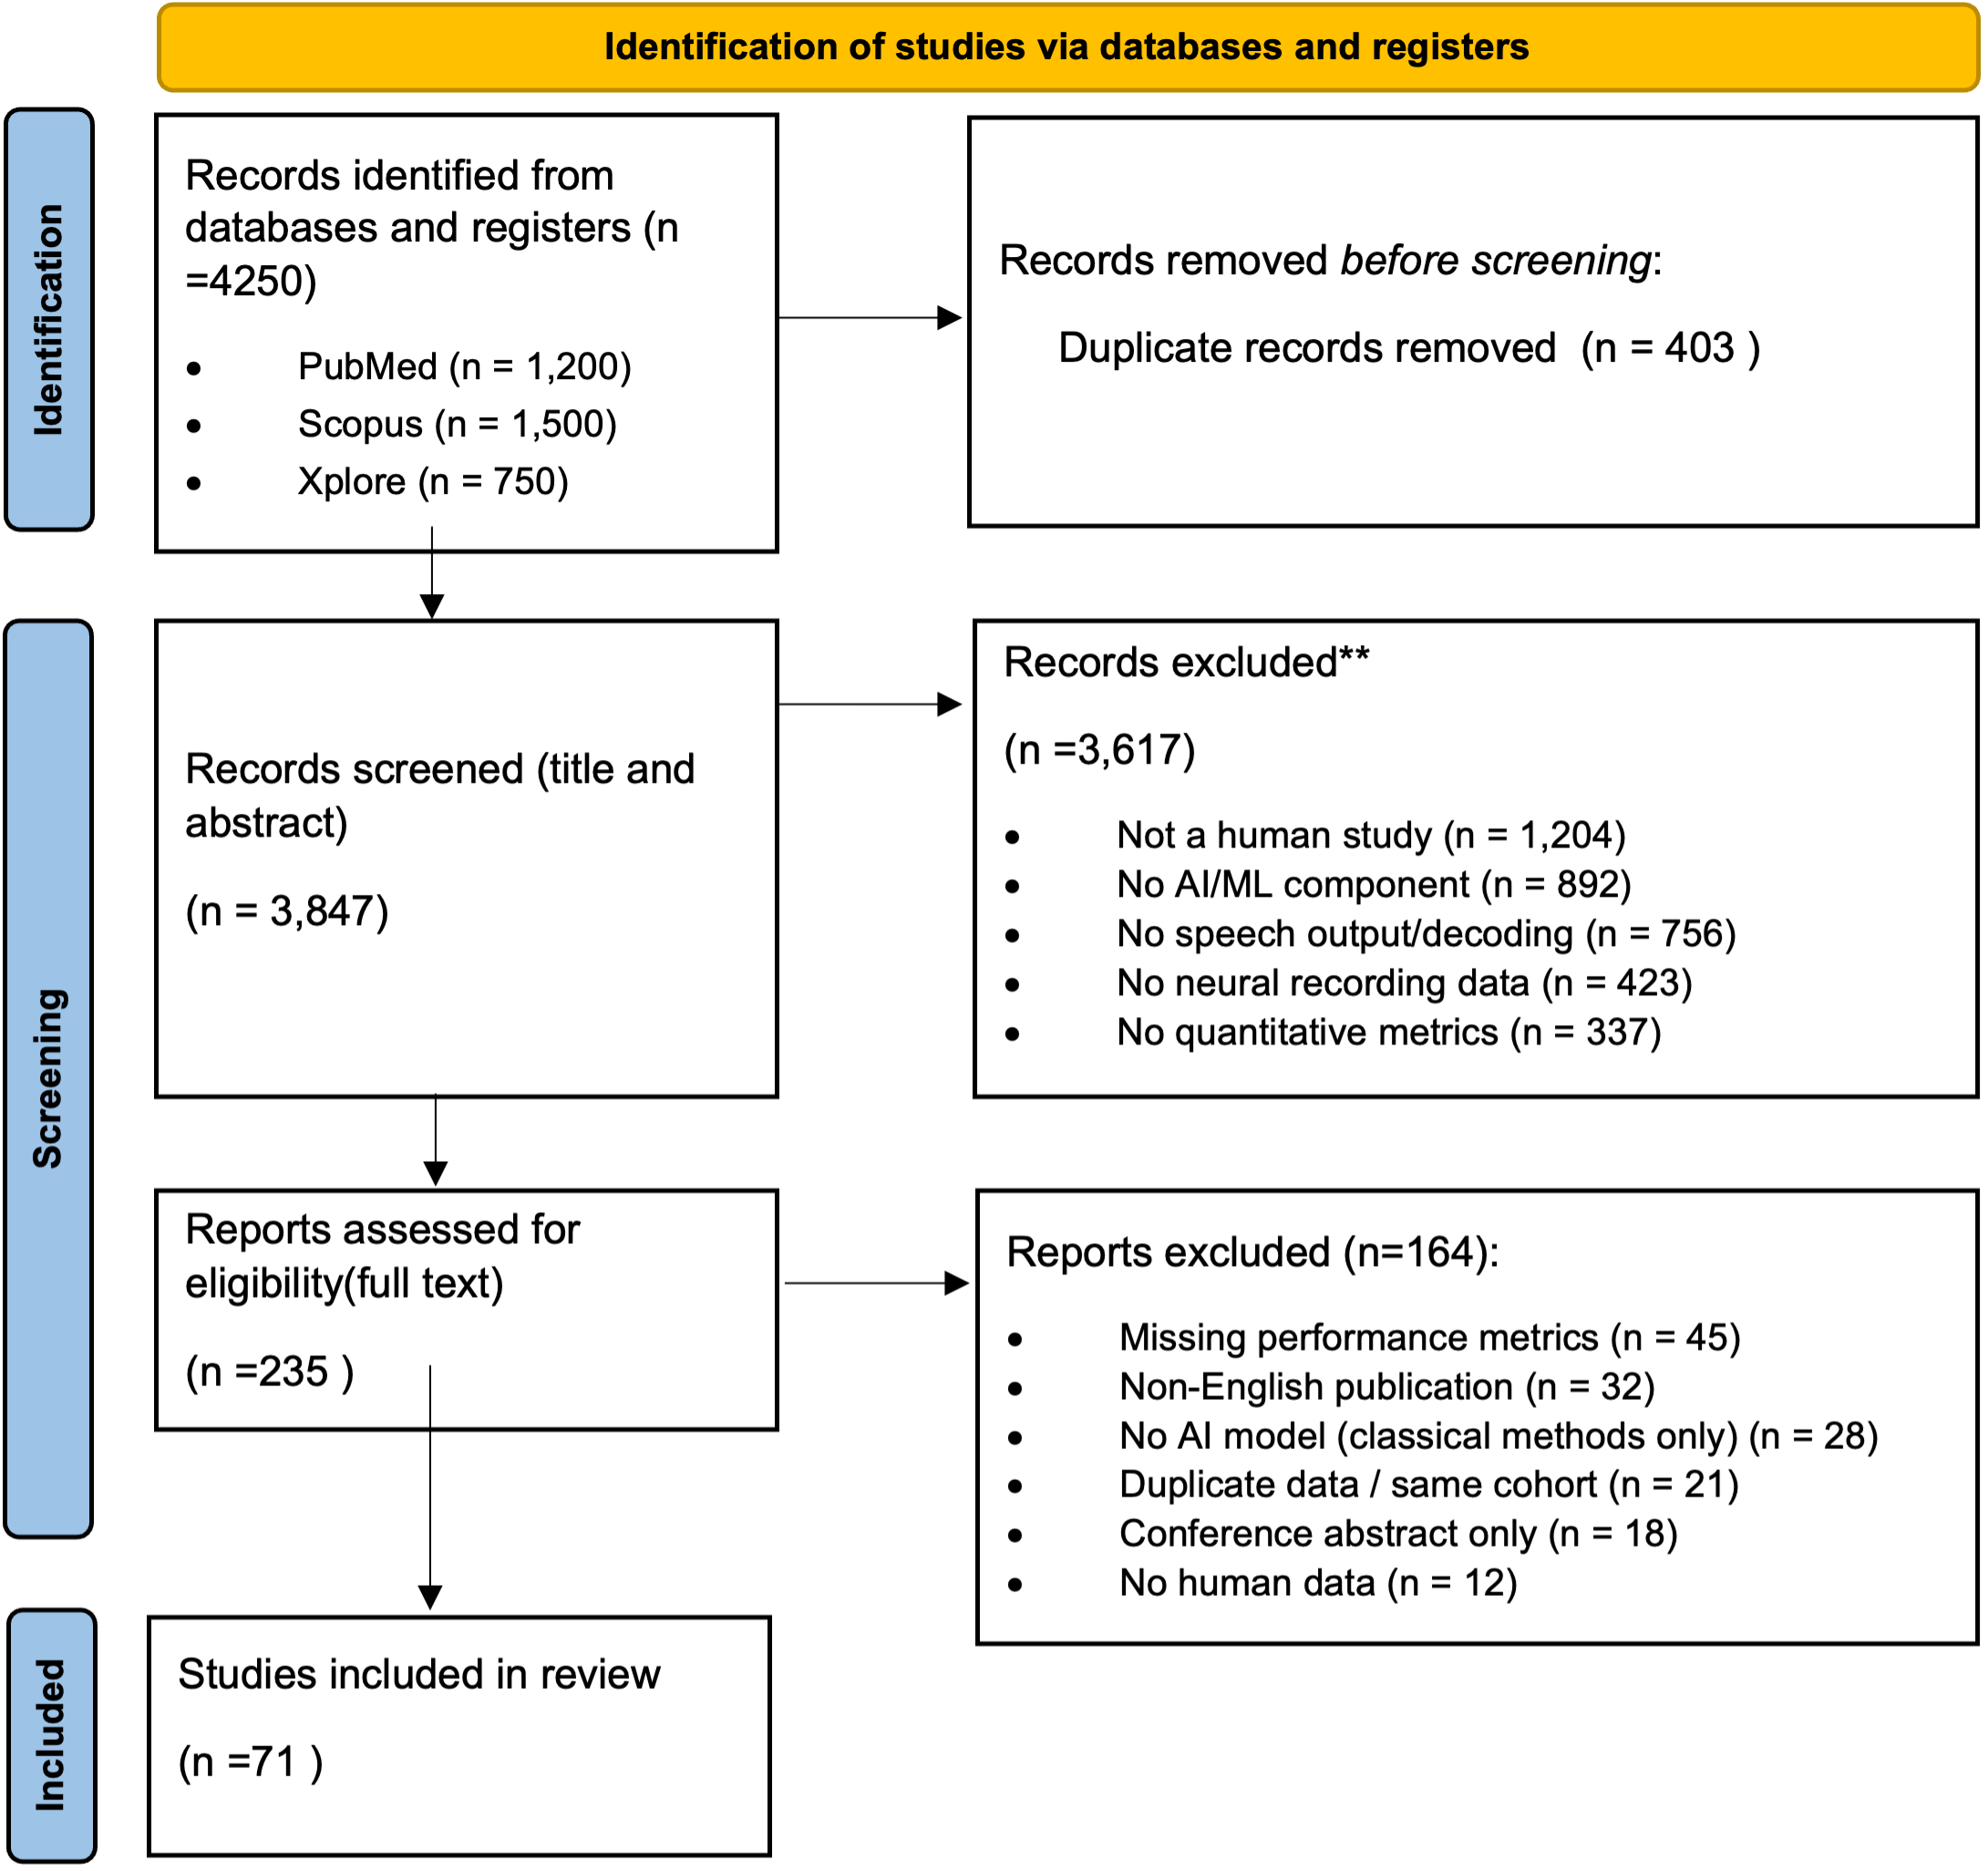
\includegraphics[width=0.95\textwidth]{figures/fig1_prisma_flow.png}
\caption{PRISMA 2020 Flow Diagram. Study selection process showing numbers at each stage: 4,250 records identified across 5 databases, 3,847 deduplicated, 235 underwent full-text assessment, 71 included in systematic review across five neural recording modality groups.}
\label{fig:prisma_flow}
\end{figure}

\vspace{2cm}

%% ============================================================================
%% FIGURE 2: STUDY DISTRIBUTION BY MODALITY AND YEAR
%% ============================================================================

\begin{figure}[h!]
\centering
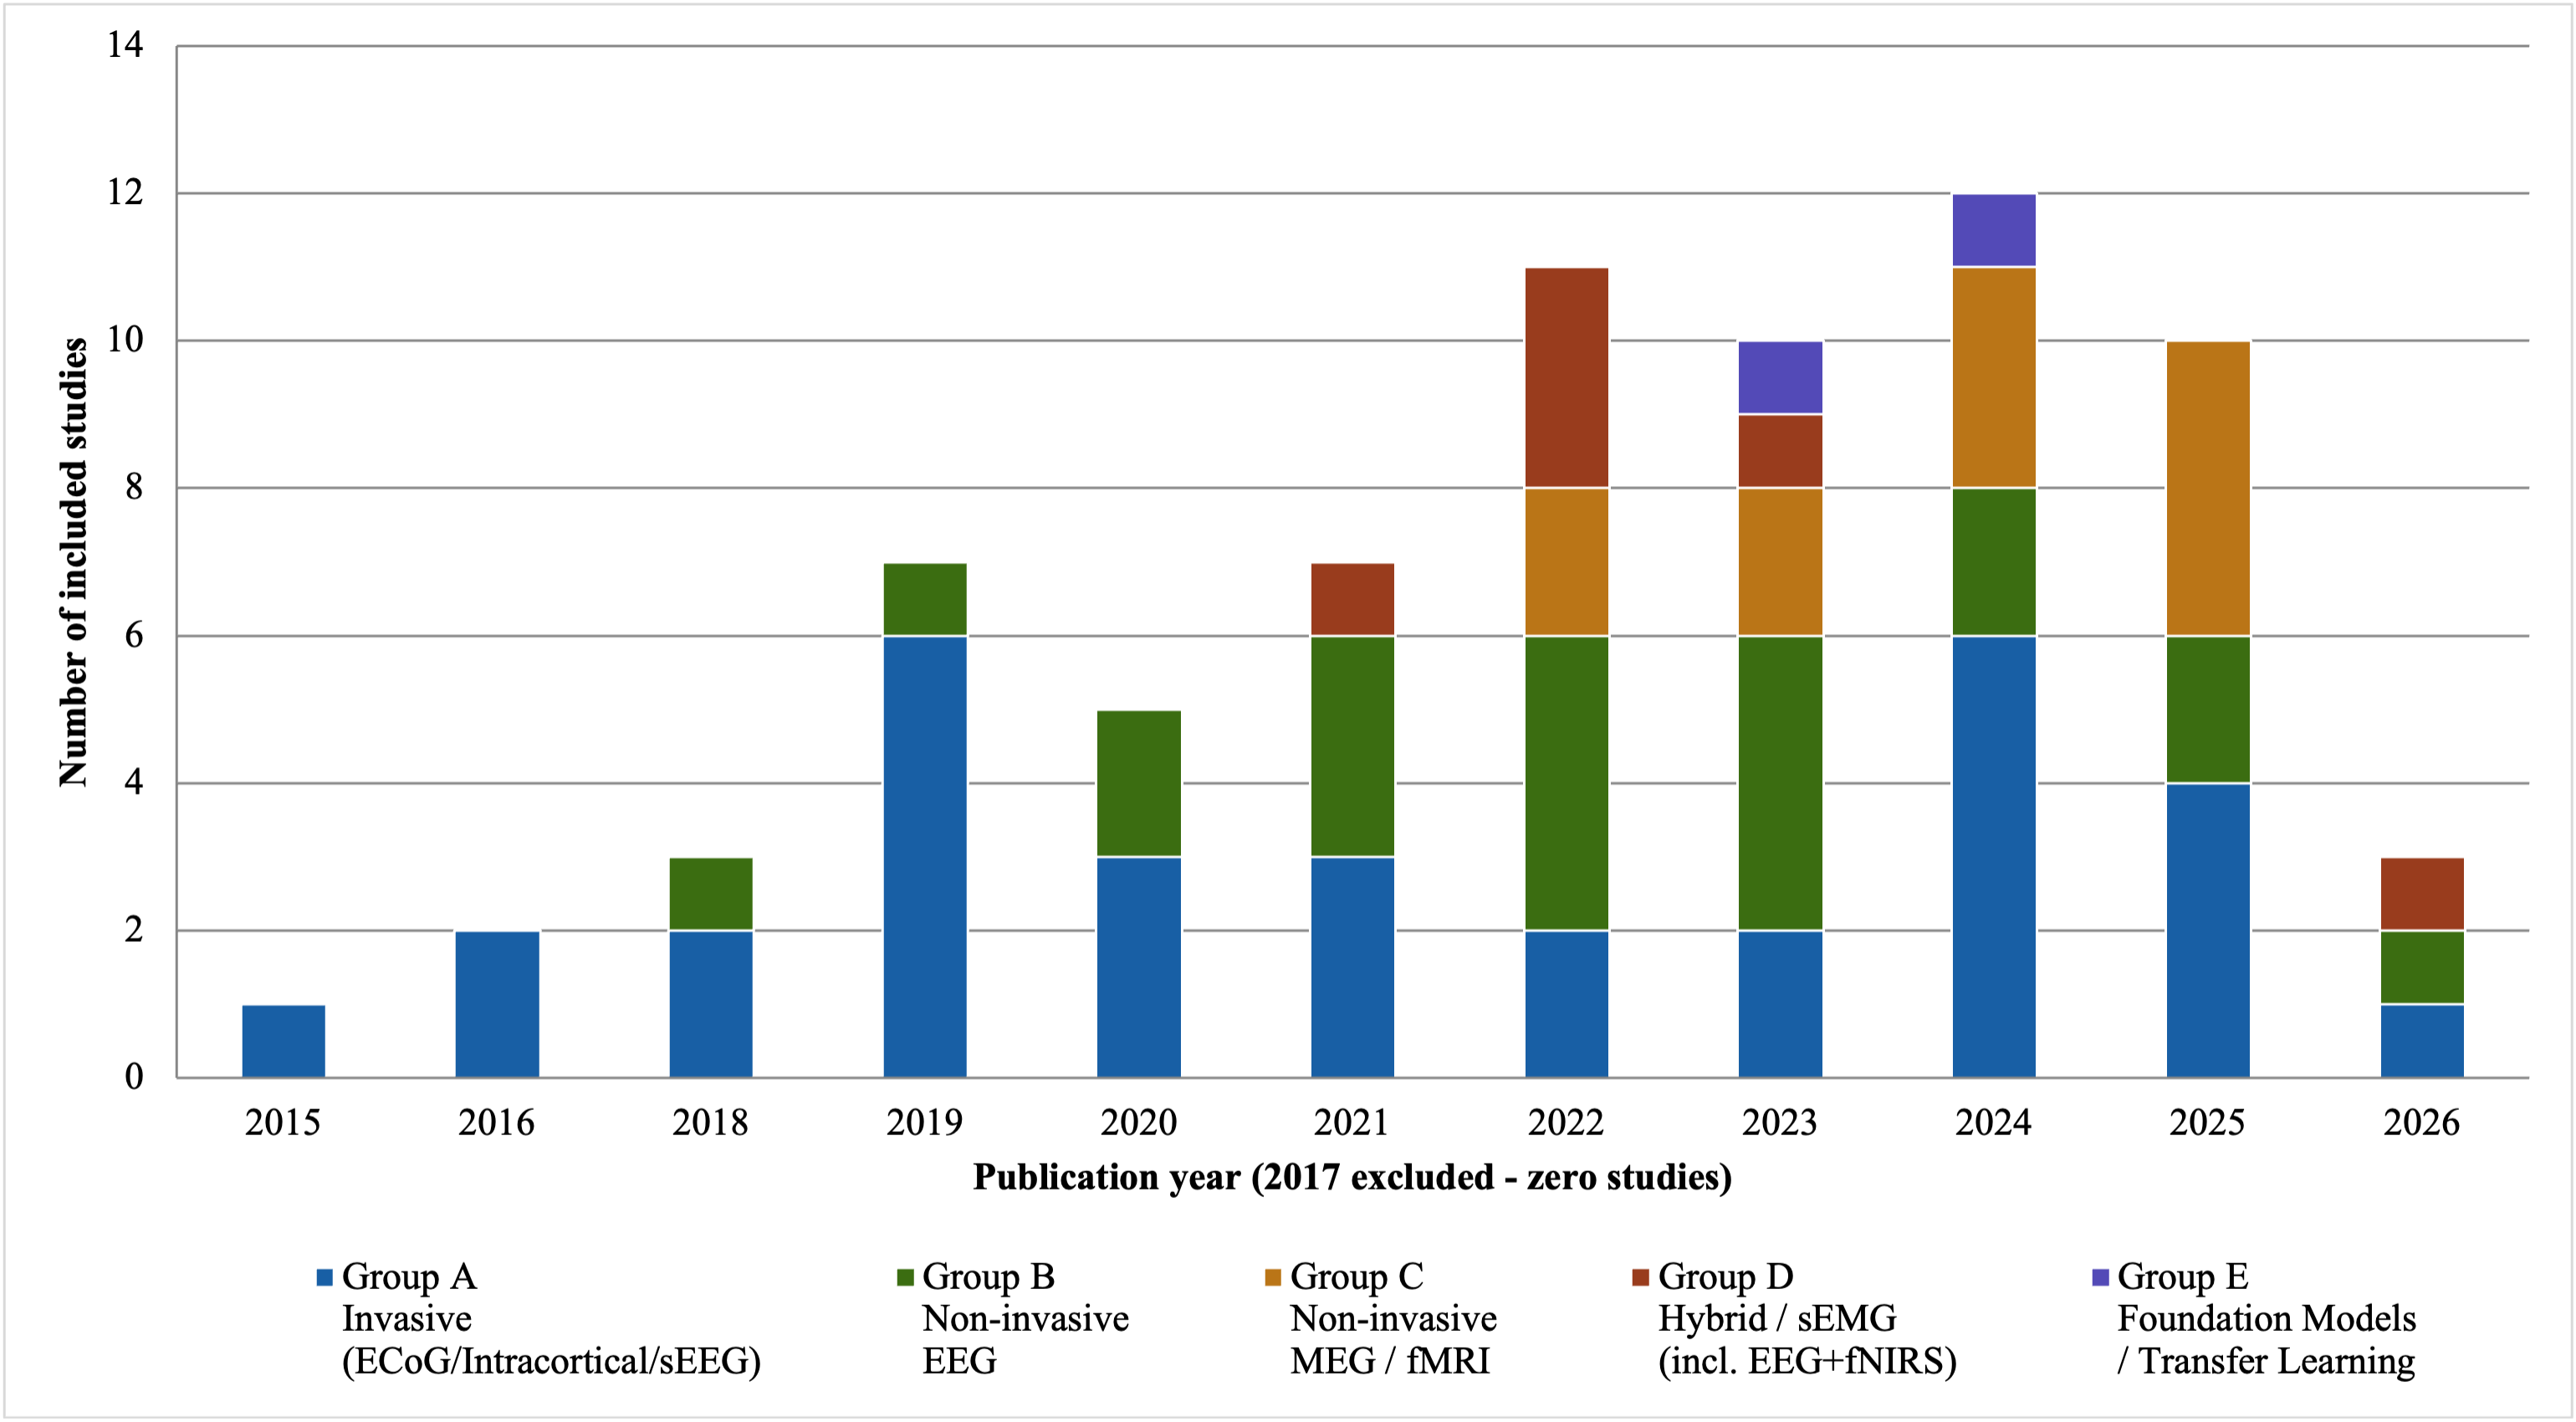
\includegraphics[width=\textwidth]{figures/fig2_study_distribution.png}
\caption{Study Distribution: 71 included studies distributed across five neural recording modality groups over the period 2015-2025. The stacked bar chart displays the temporal distribution of publications by modality type. Growth in non-invasive modality publications is visible from 2022 onwards, concurrent with transformer architecture adoption and self-supervised learning emergence.}
\label{fig:study_distribution}
\end{figure}

%% ============================================================================
%% FIGURE 3: AI ARCHITECTURE EVOLUTION AND CHRONOLOGICAL TRANSITION (2015-2026)
%% ============================================================================

\begin{figure}[h!]
\centering
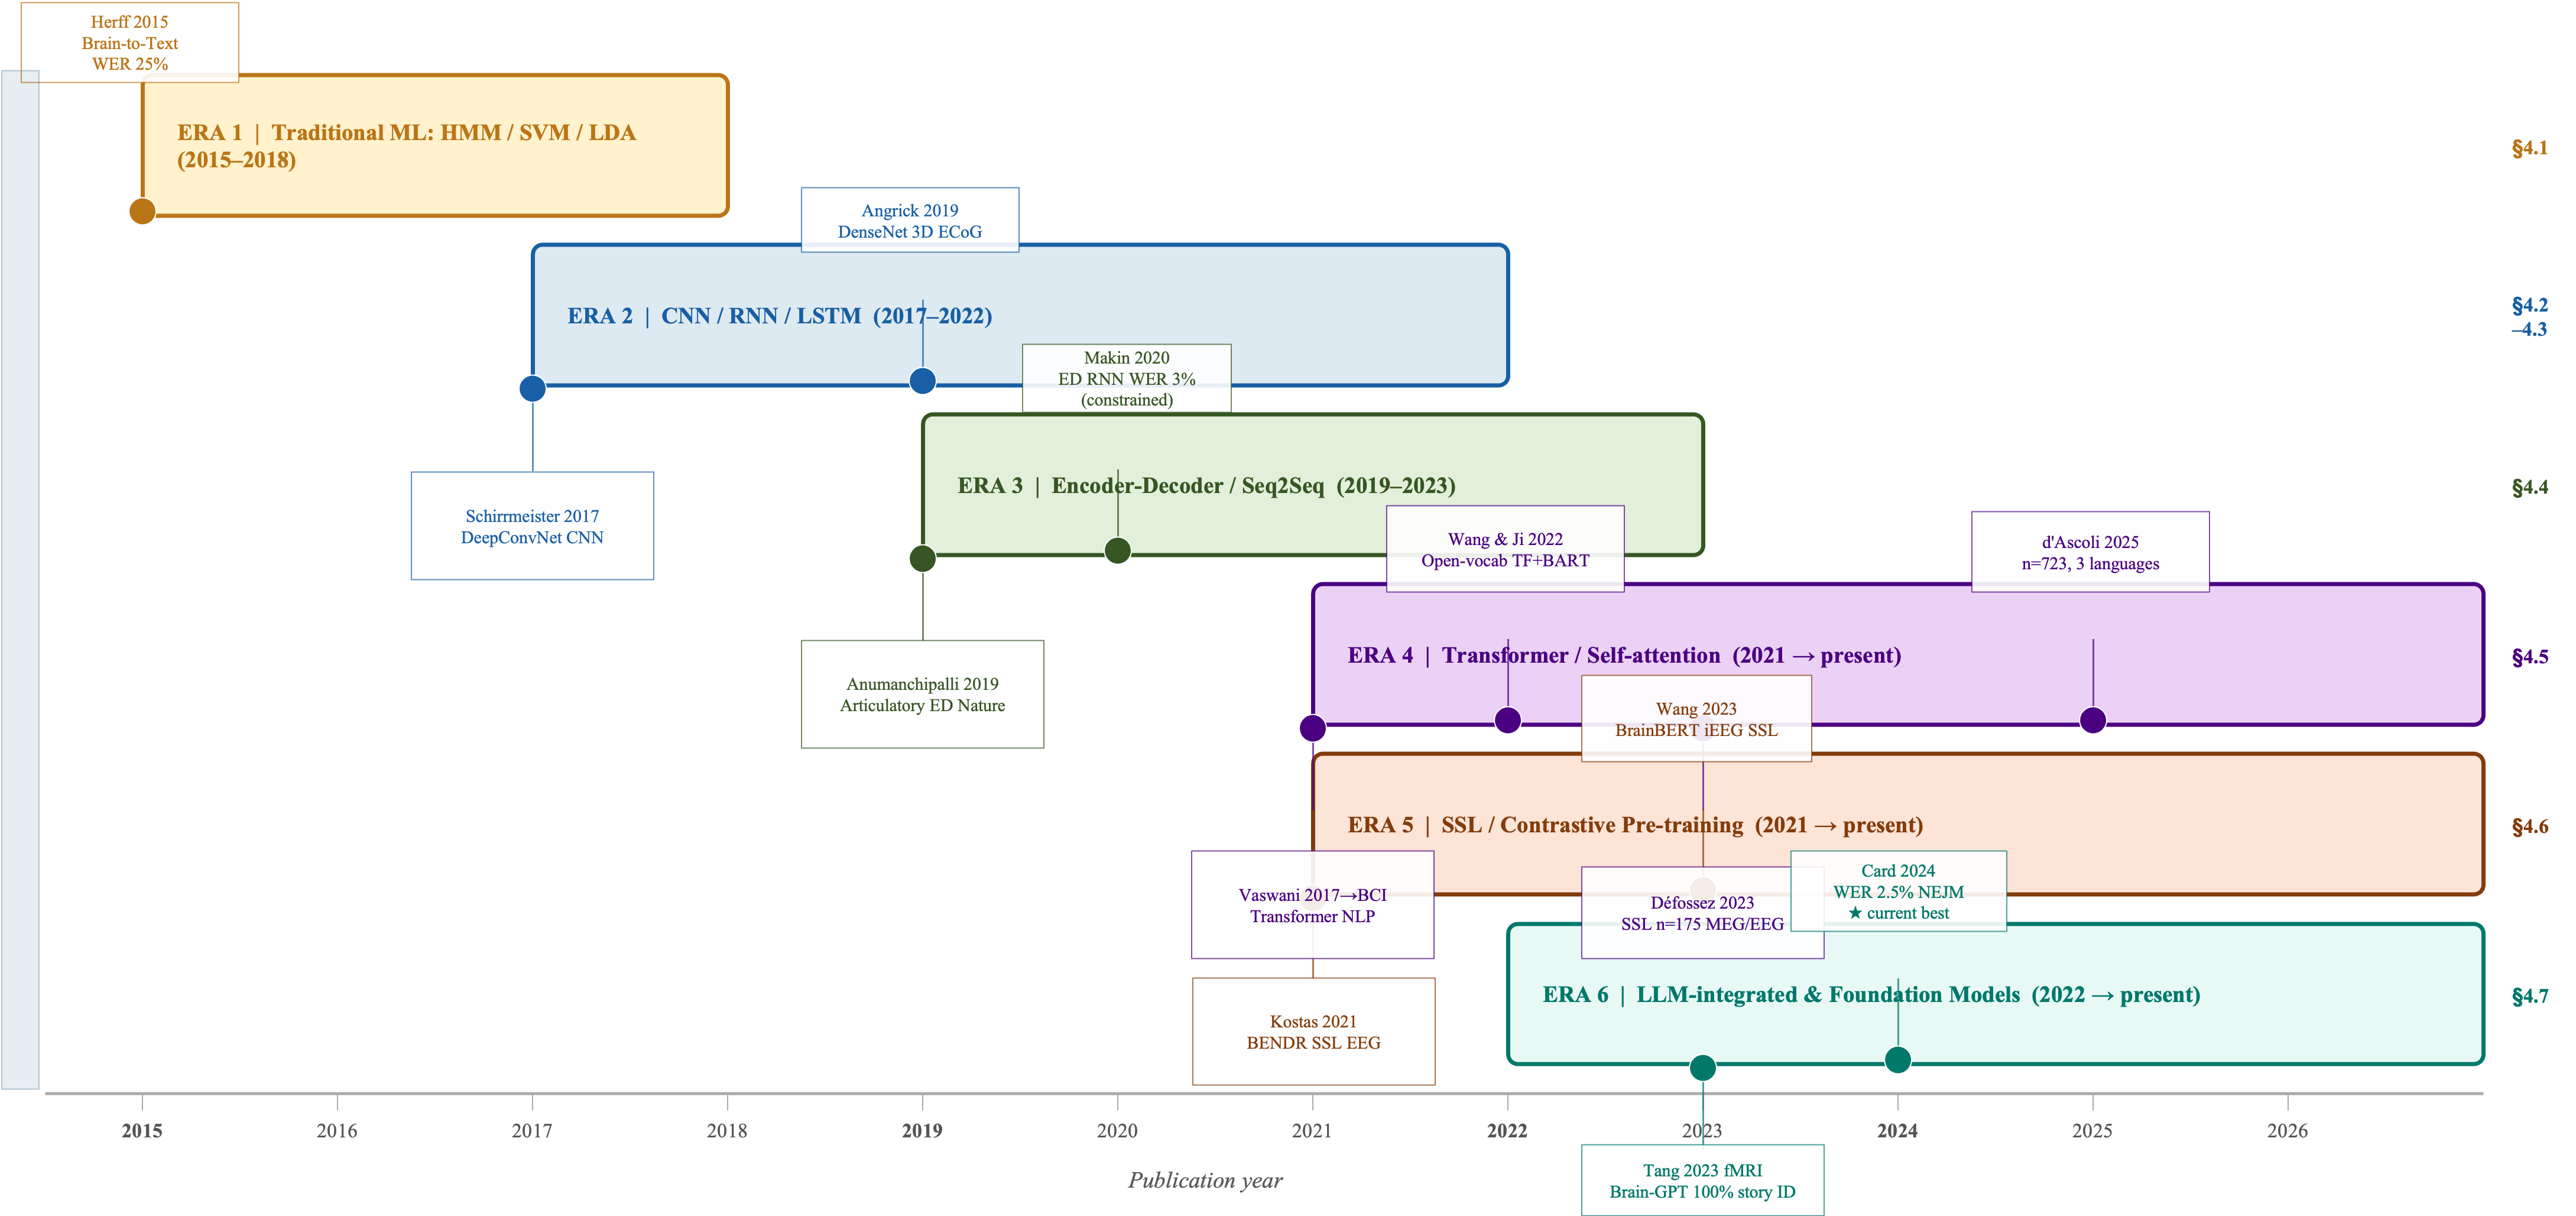
\includegraphics[width=\textwidth]{figures/fig3_architecture_evolution.png}
\caption{AI Architecture Evolution: Chronological transition across eight architecture classes (2015-2026). Traditional machine learning (2015-2018) gave way to convolutional neural networks (2017-2022), recurrent networks/LSTMs (2018-2023), and encoder-decoder systems (2019-2022). Transformer architectures (2022-present) and self-supervised learning (2021-present) dominate recent studies, while LLM-integrated approaches (2022-present) represent the fastest-growing category. Height of bars indicates relative proportion of included studies; color indicates dominant period of adoption.}
\label{fig:architecture_evolution}
\end{figure}

%% ============================================================================
%% FIGURE 4: WER PERFORMANCE TRAJECTORY (LANDMARK STUDIES)
%% ============================================================================

\begin{figure}[h!]
\centering
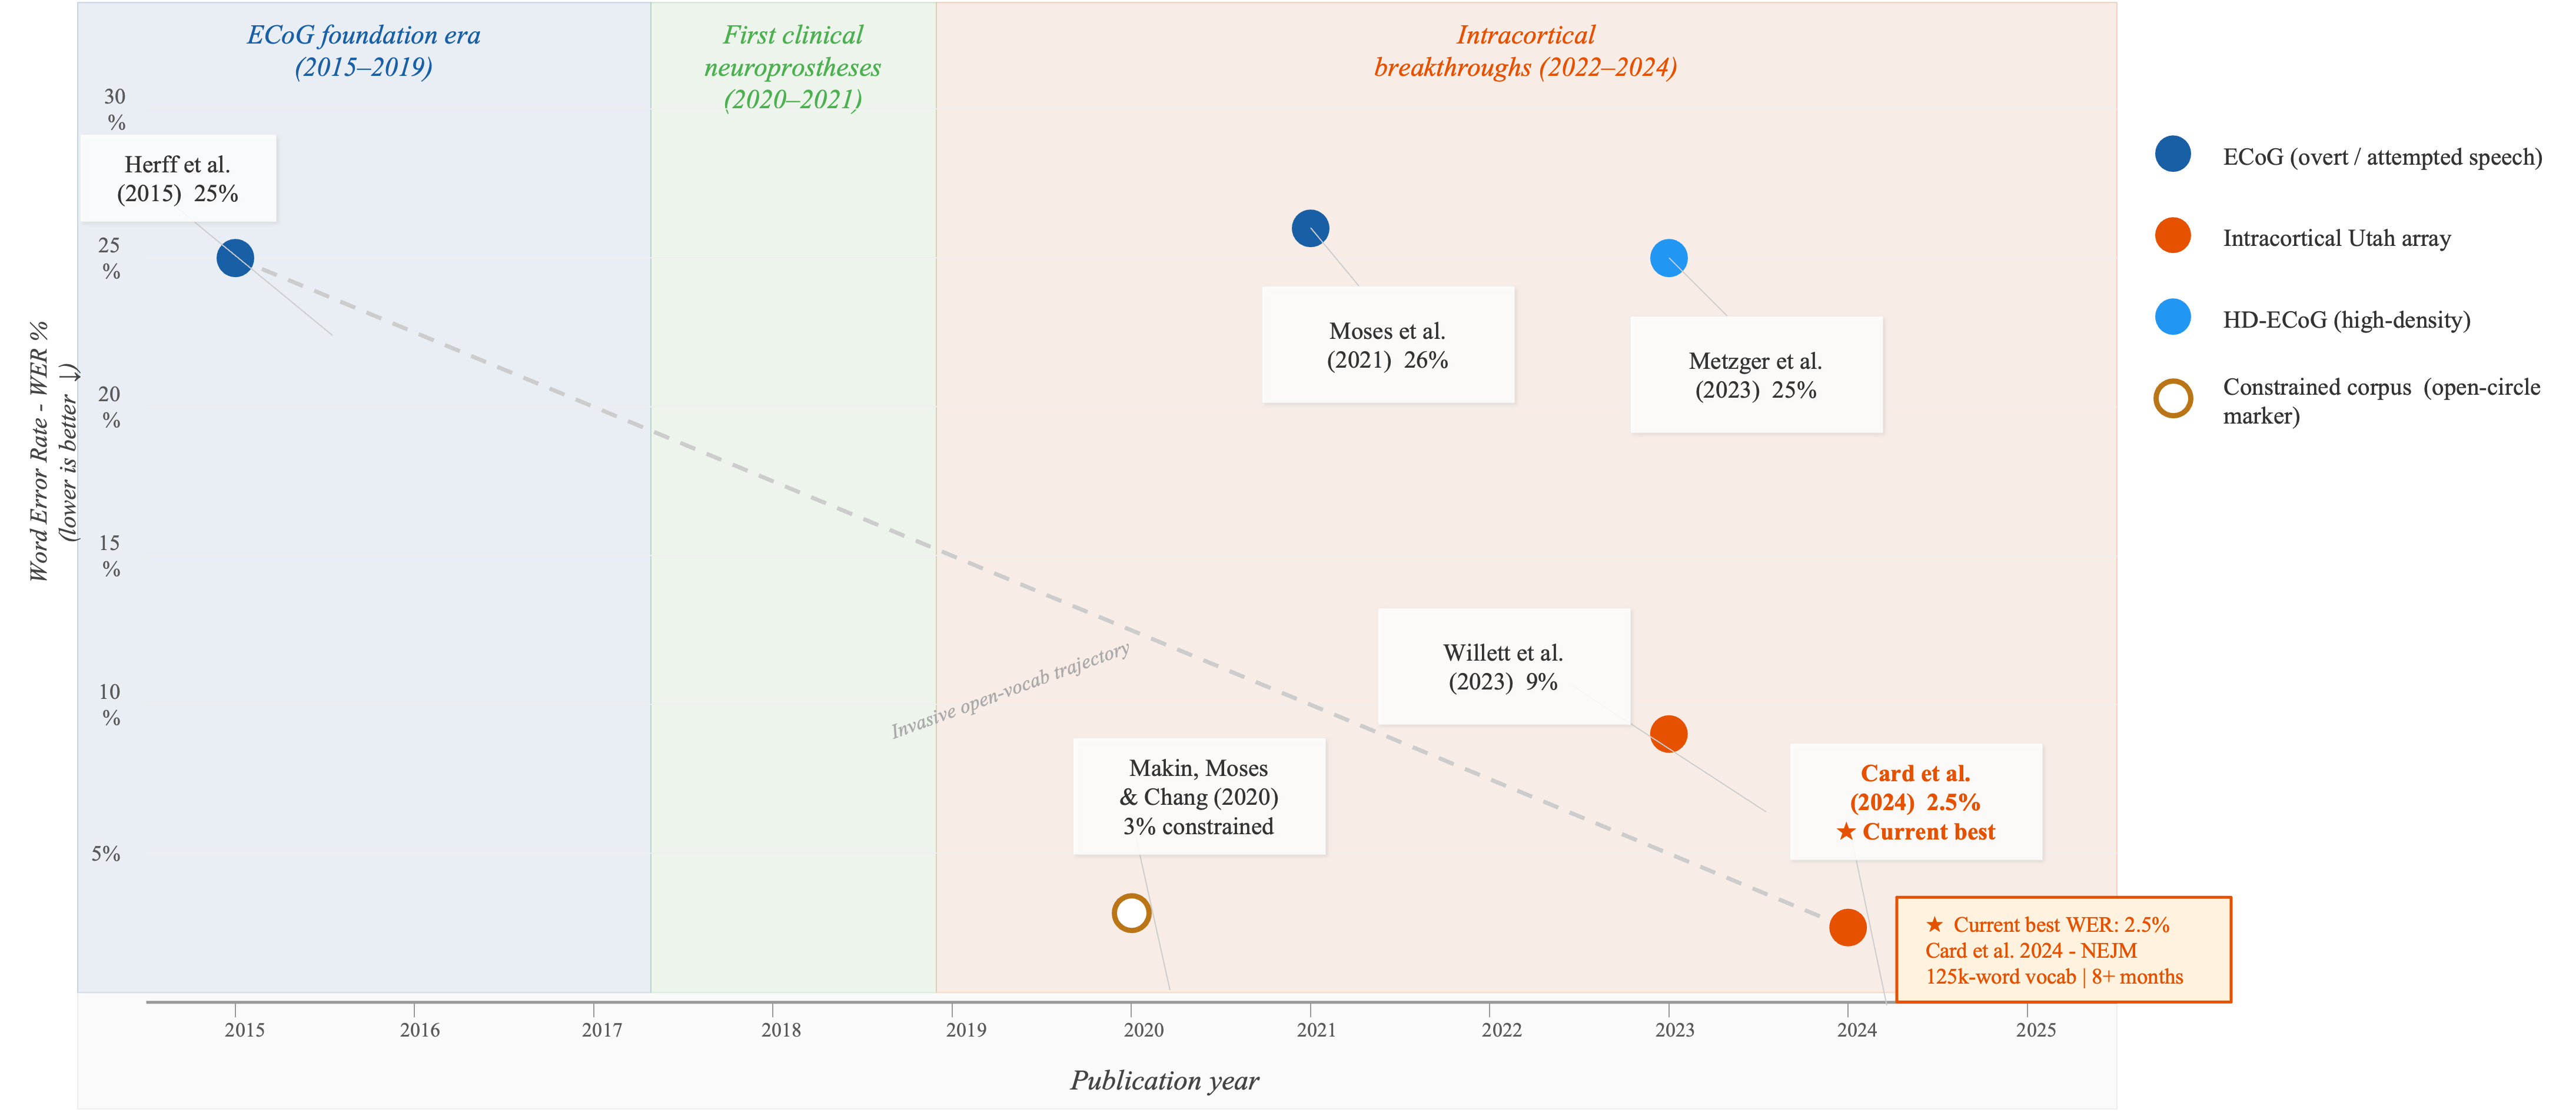
\includegraphics[width=\textwidth]{figures/fig4_wer_trajectory.png}
\caption{WER Performance Trajectory: Landmark invasive systems show progression from 2015-2024. Herff et al. (2015): 25\% WER on ECoG with 7 participants; Moses et al. (2021): 15.2 WPM with intracortical; Willett et al. (2023): 9\% WER (50-word) with intracortical; Card et al. (2024): 2.5\% WER (125k-word) with intracortical. Trajectory demonstrates the cumulative effect of improved electrode technology, deep learning architectures, and language model integration. Single-participant studies dominate recent years, reflecting shift toward intensive optimization on individual cases.}
\label{fig:wer_trajectory}
\end{figure}

%% ============================================================================
%% FIGURE 5: MODALITY × TASK PERFORMANCE HEATMAP
%% ============================================================================

\begin{figure}[h!]
\centering
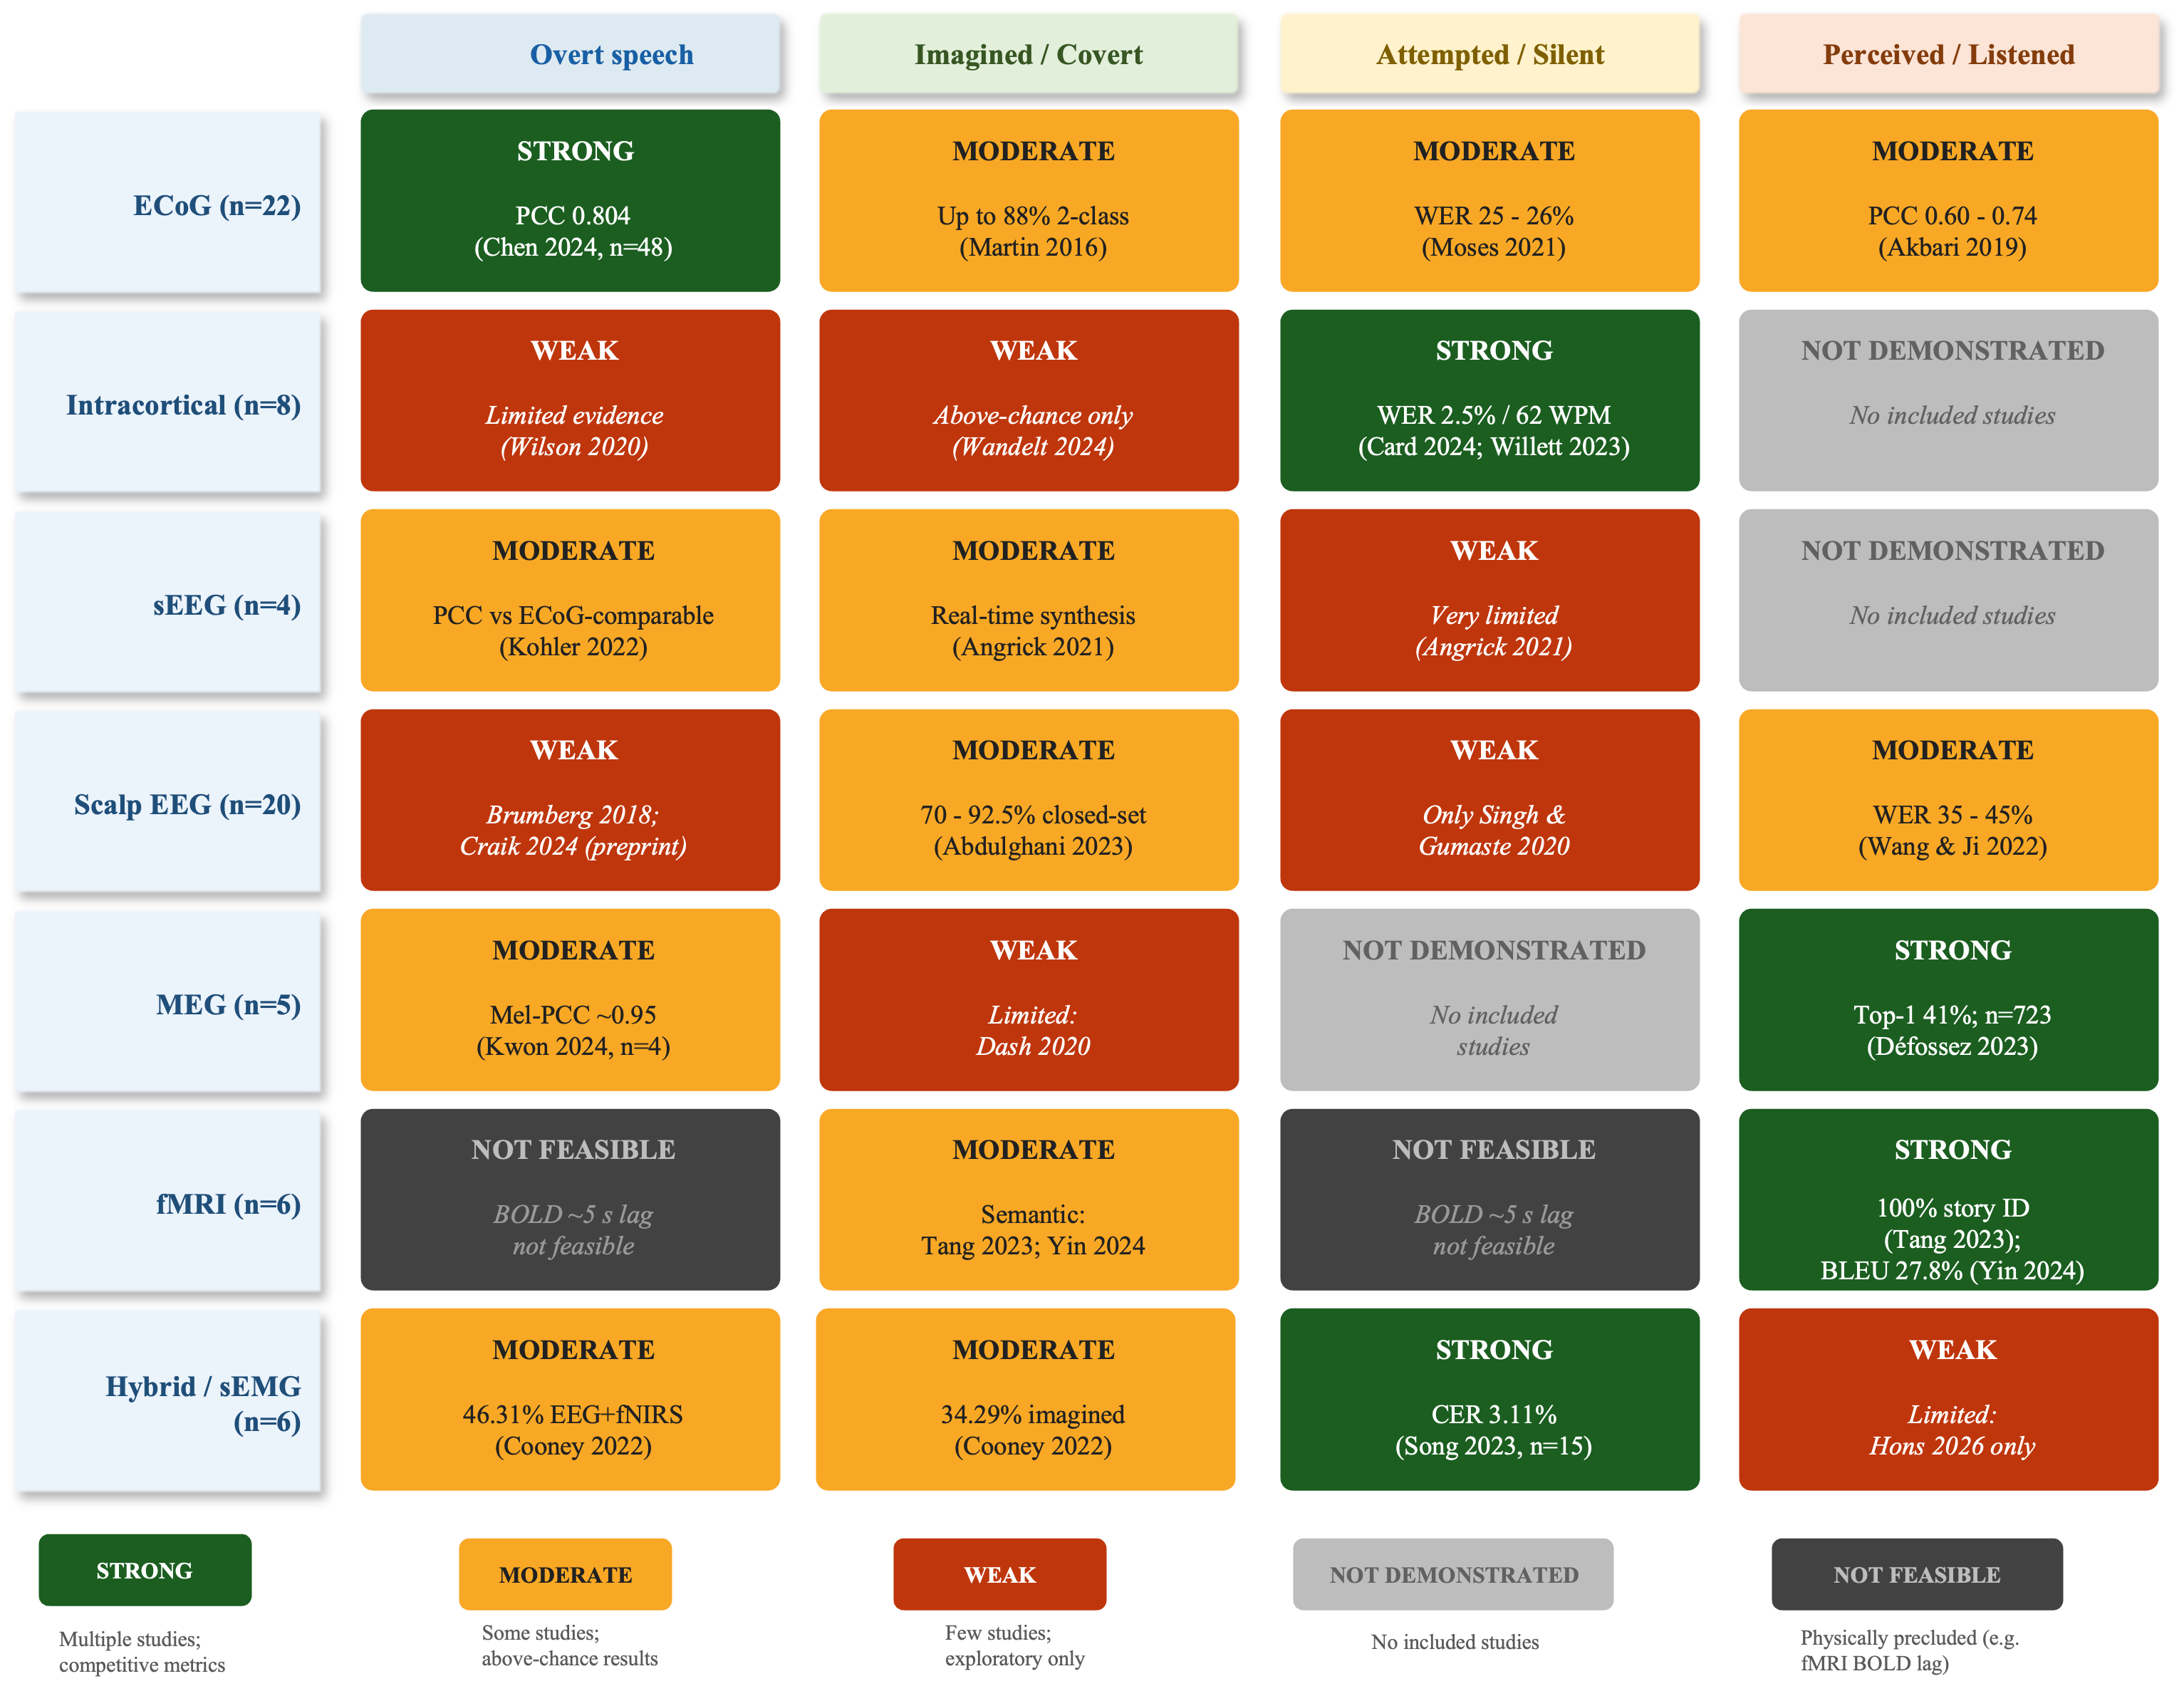
\includegraphics[width=\textwidth]{figures/fig5_modality_task_heatmap.png}
\caption{Modality × Task Performance Heatmap: Neural recording modality groups (rows) versus task type categories (columns) with color-coded performance levels. The heatmap reveals performance gradients: invasive modalities (ECoG, intracortical, sEEG) demonstrate strong performance across all task types; non-invasive modalities (EEG, MEG, fMRI) cluster in lower-performance regions for real-time decoding tasks, with fMRI strong only for semantic reconstruction. Performance varies systematically: closed-set classification achieves 70-99\% across all modalities; open-vocabulary continuous speech shows 3-10x variation. Warm colors indicate higher performance; cool colors indicate lower performance.}
\label{fig:modality_task_heatmap}
\end{figure}

\clearpage

%% ============================================================================
%% FIGURE 6: MODALITY COMPARISON MATRIX (SPATIAL VS TEMPORAL RESOLUTION)
%% ============================================================================

\begin{figure}[h!]
\centering
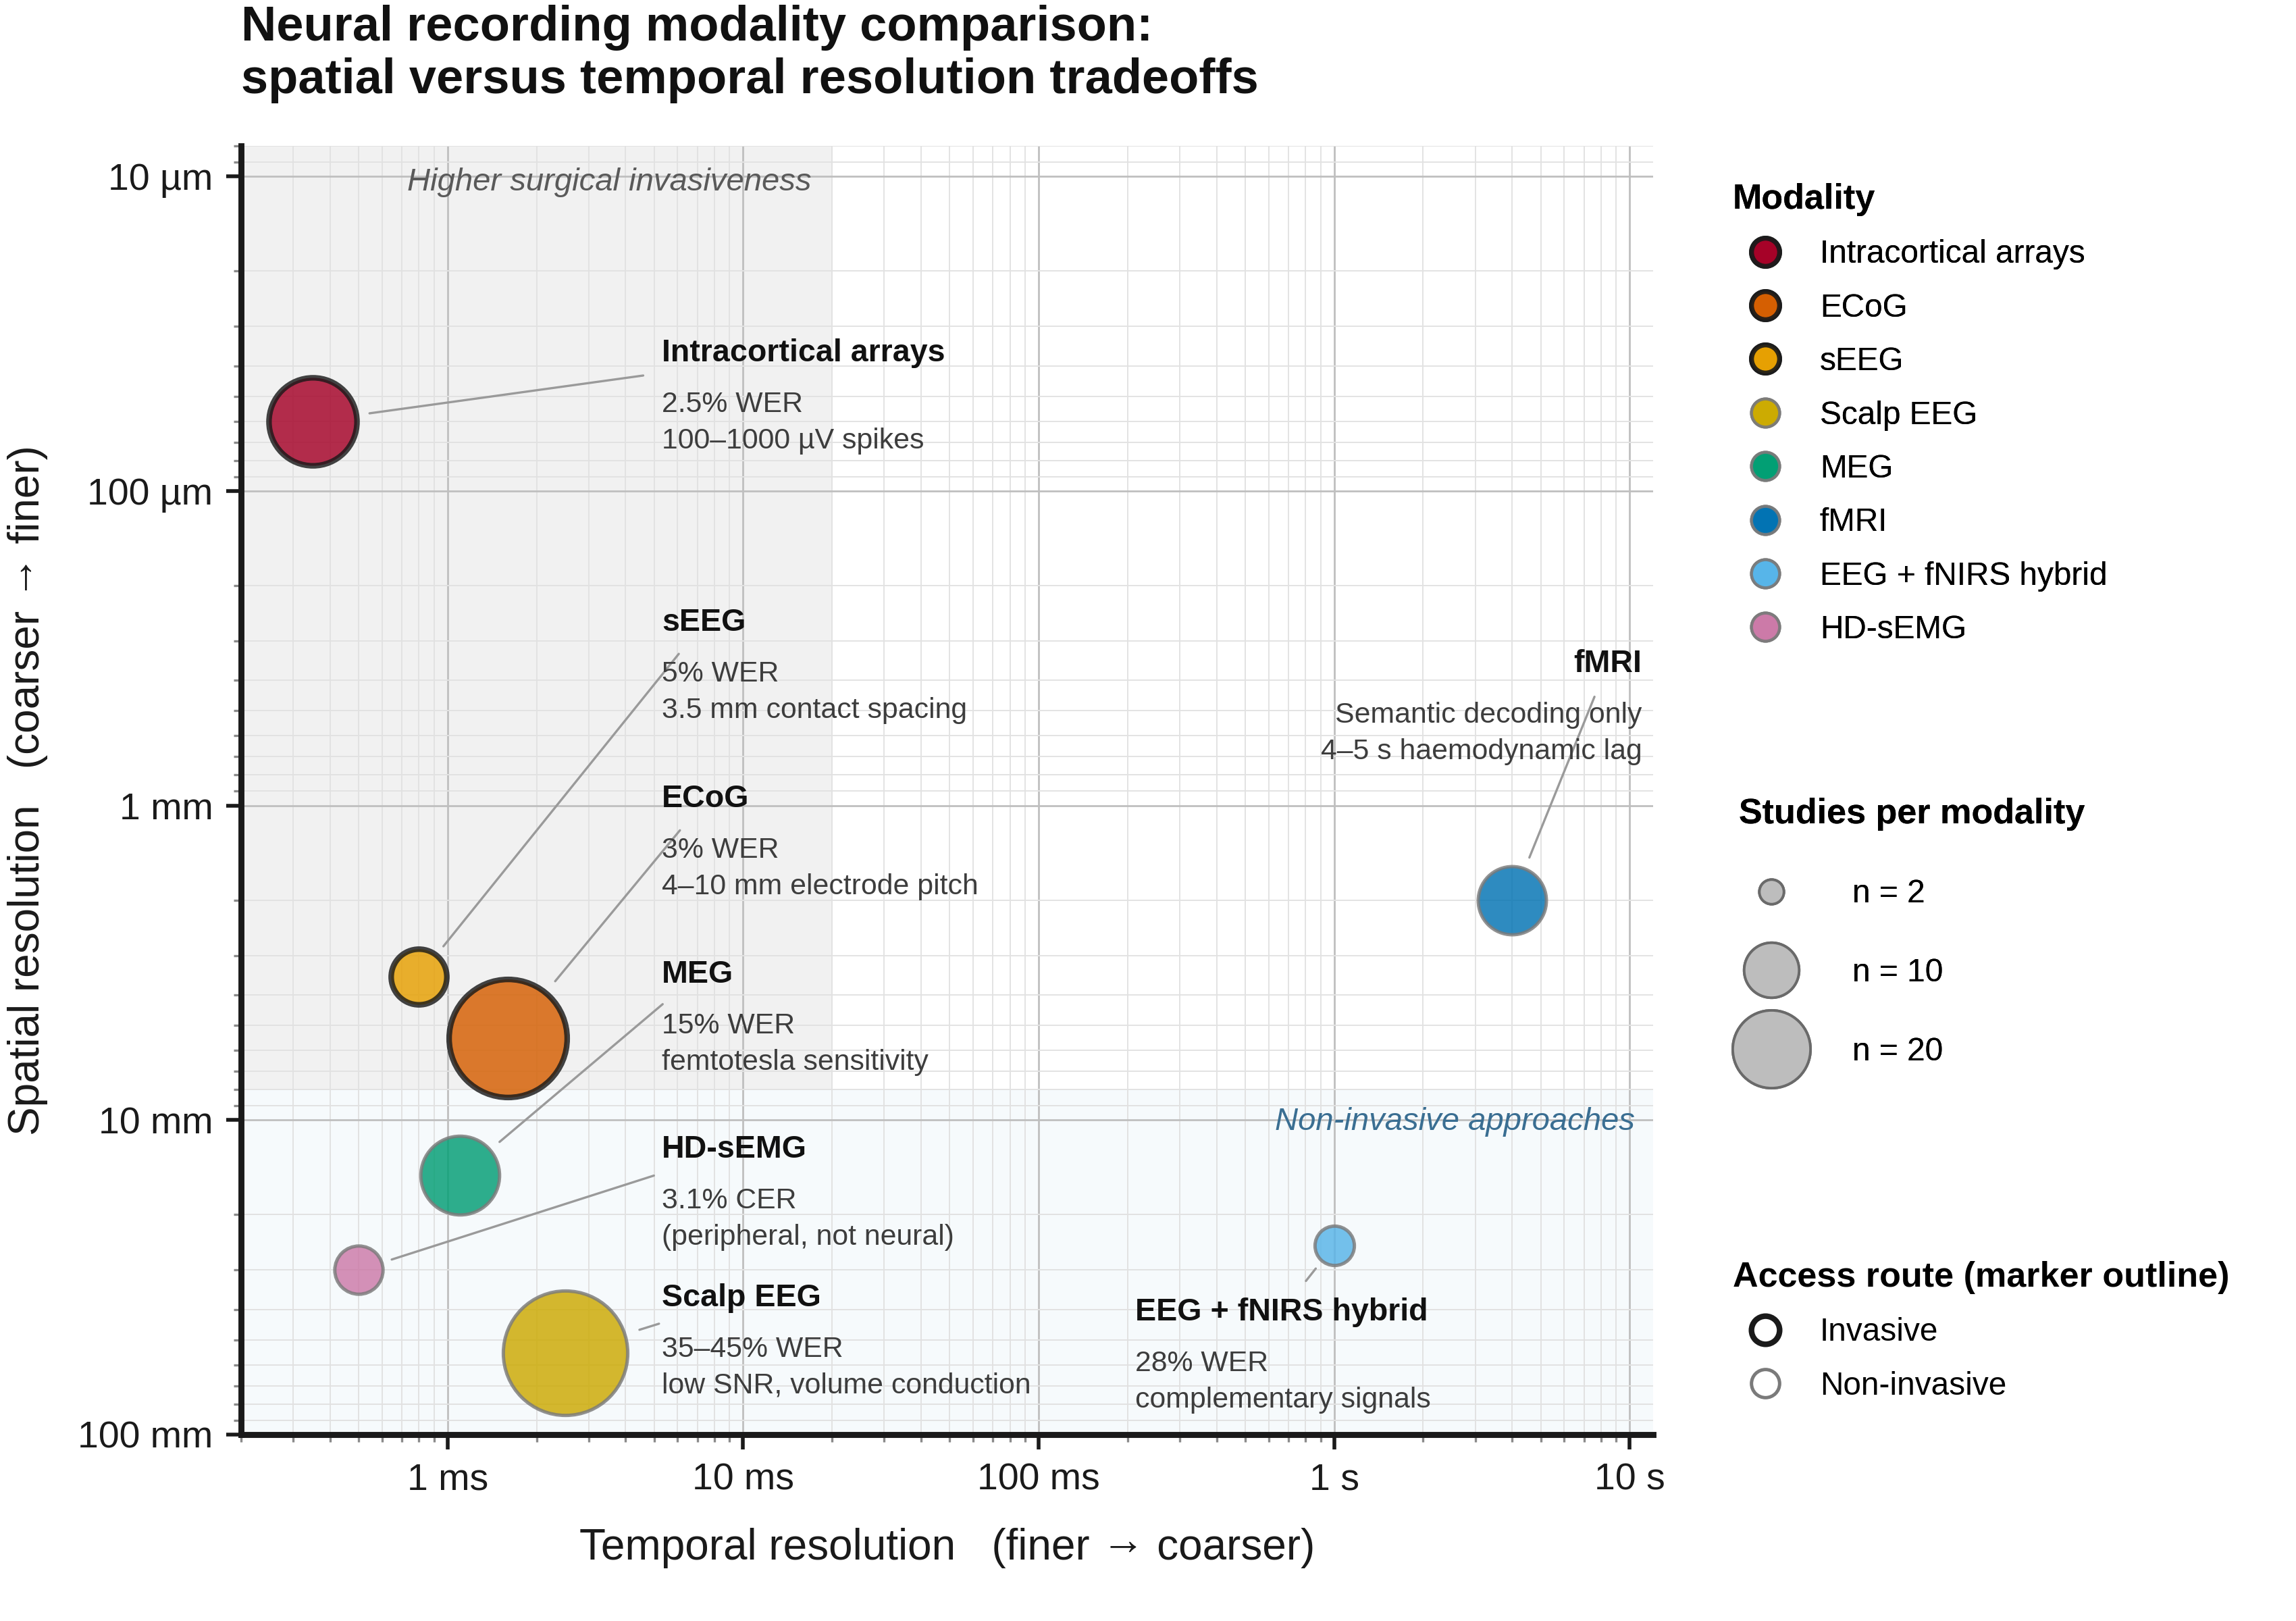
\includegraphics[width=0.95\textwidth]{figures/fig6_modality_comparison.png}
\caption{Modality Comparison Matrix: Spatial versus temporal resolution tradeoffs across eight primary neural recording modalities (invasive ECoG, intracortical, sEEG; non-invasive EEG, MEG, fMRI; hybrid EEG+fNIRS, HD-sEMG). Each circle represents one modality; circle size indicates typical study count. The upper-right corner (fine spatial, fine temporal) is unattainable due to fundamental physics constraints. Invasive modalities (red/orange) dominate the upper-left (fine temporal, variable spatial); non-invasive modalities spread across lower quadrants. fMRI uniquely occupies upper-right (fine spatial, coarse temporal), trading temporal fidelity for whole-brain coverage.}
\label{fig:modality_matrix}
\end{figure}

\vspace{1.5cm}

%% ============================================================================
%% FIGURE 7: RECORDING ELECTRODE TYPES AND PLACEMENT SCHEMATICS
%% ============================================================================

\begin{figure}[h!]
\centering
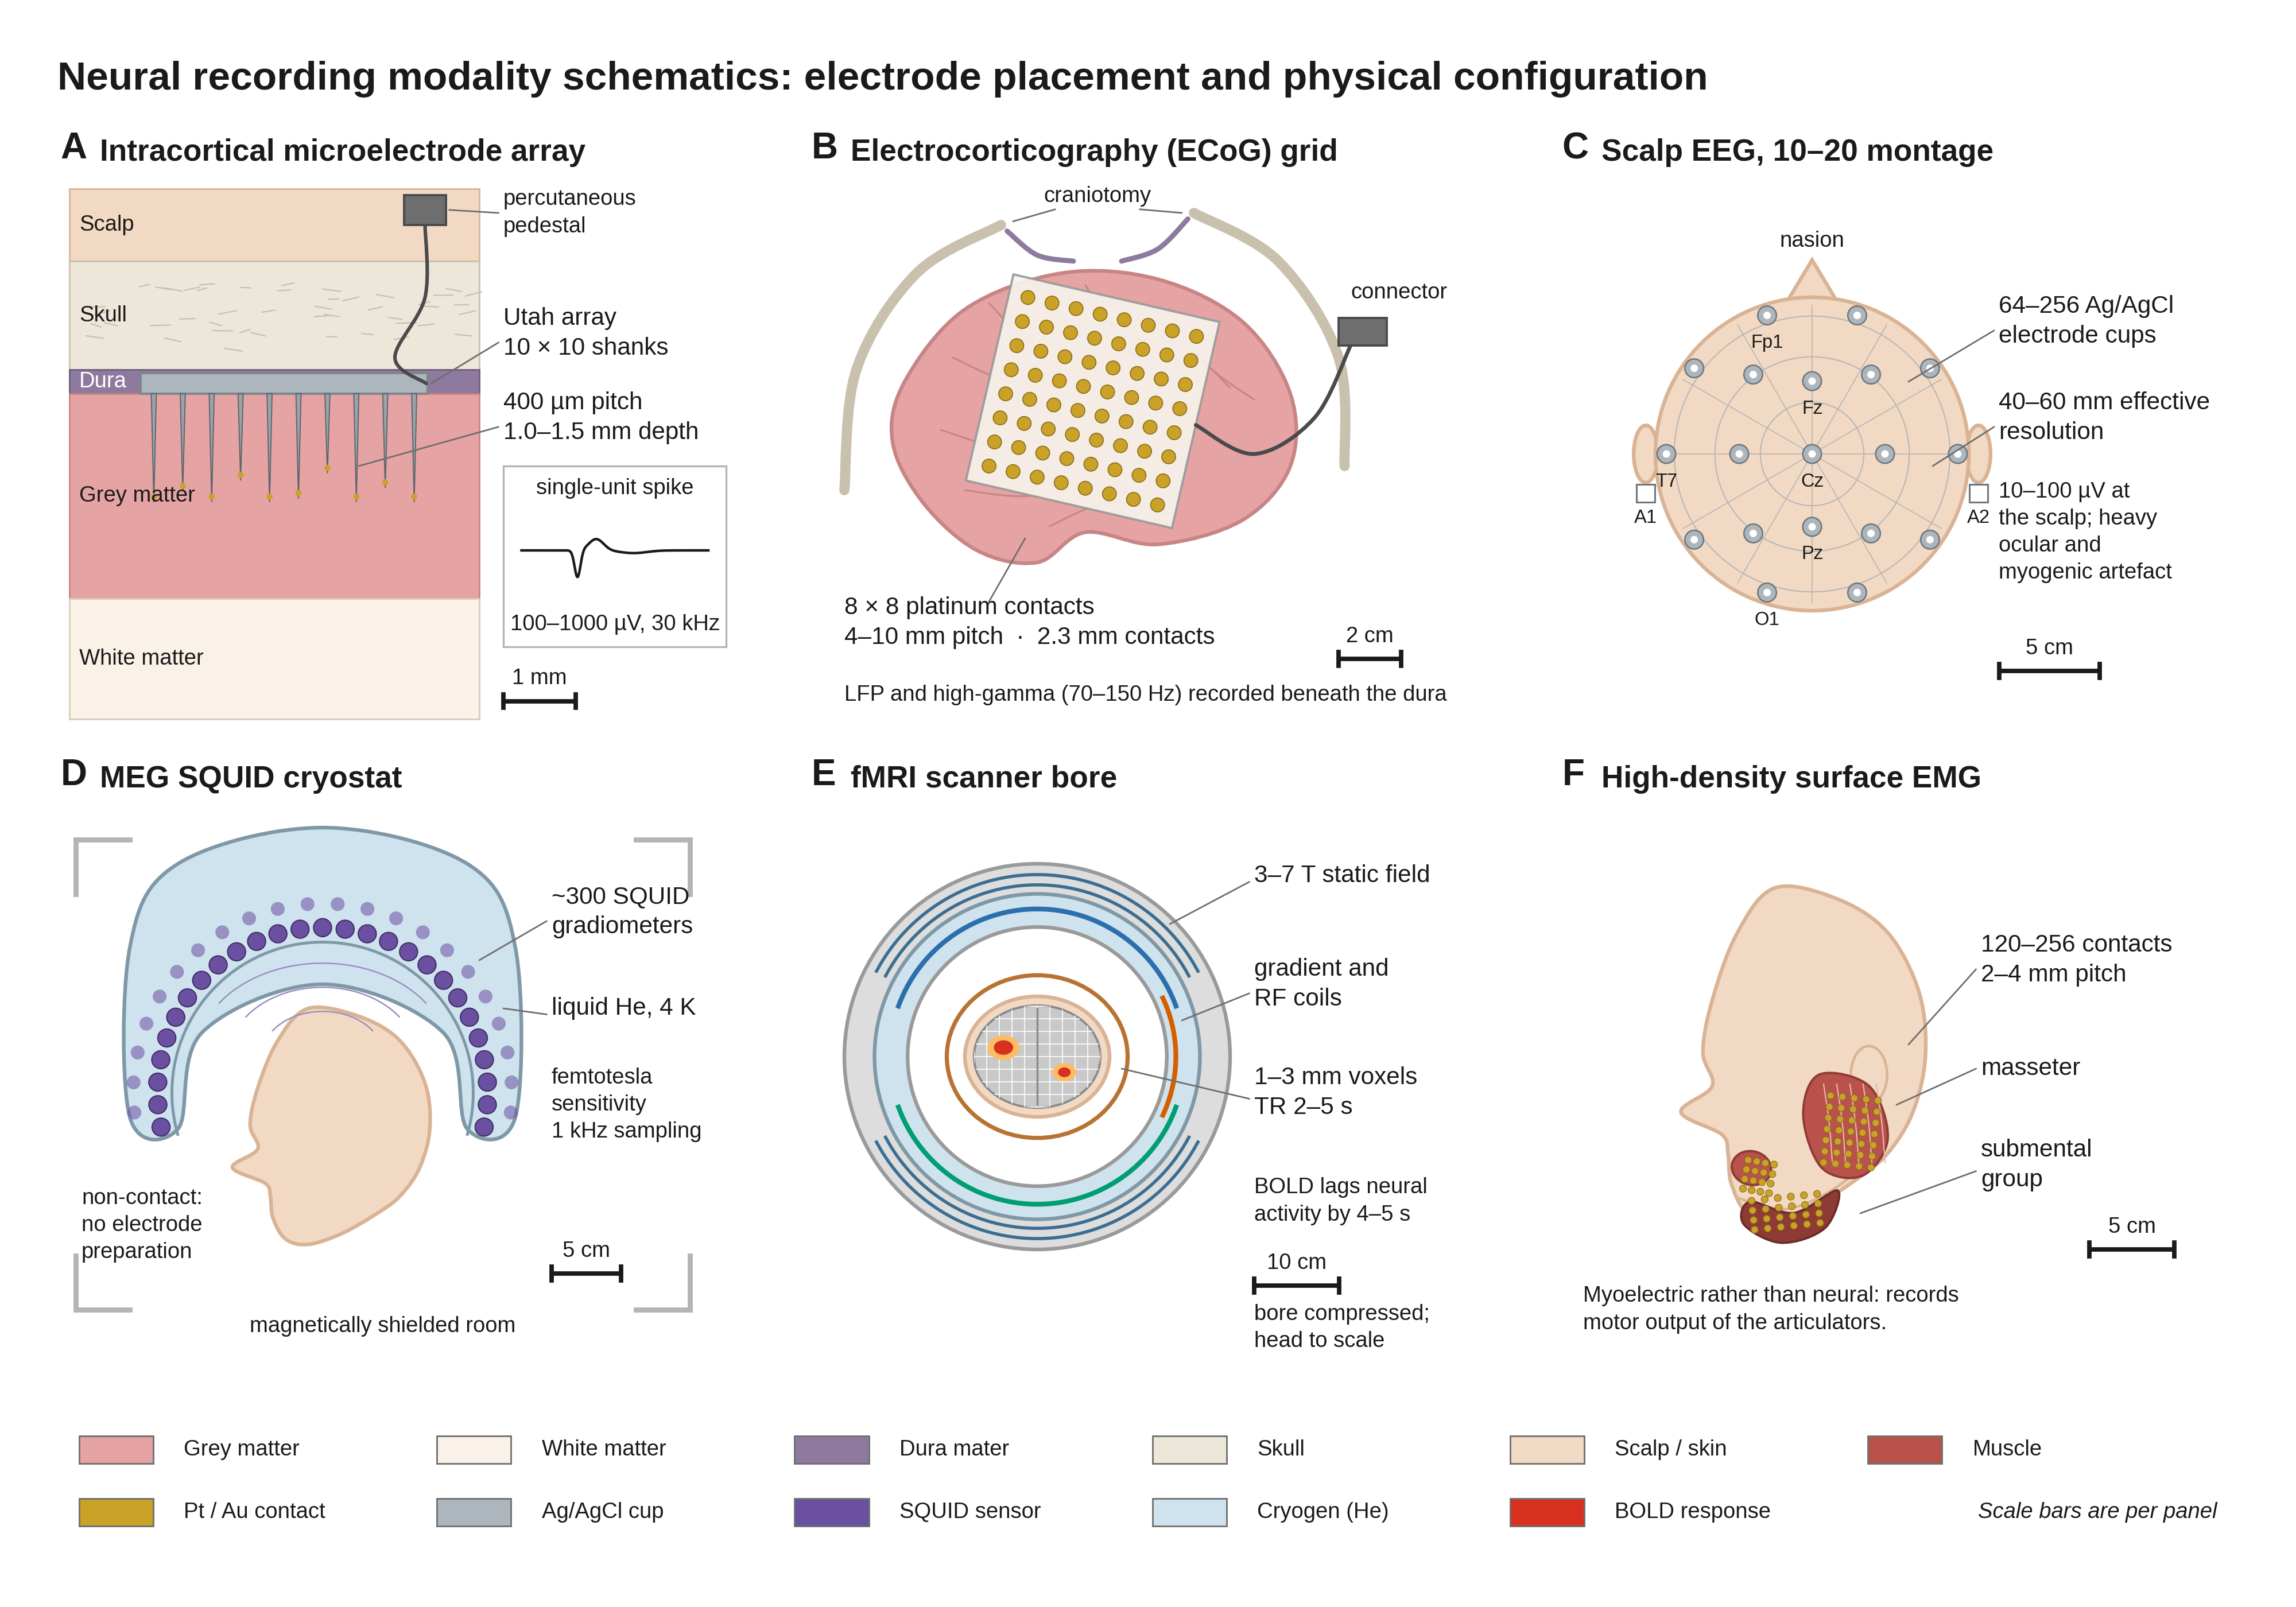
\includegraphics[width=0.98\textwidth]{figures/fig7_modality_schematics.png}
\caption{Neural Recording Modality Schematics: Six panels (A-F) showing electrode placement and physical characteristics of major recording modalities used in brain-to-speech decoding. (A) Intracortical microelectrode arrays penetrate gray matter for single-unit recording. (B) ECoG grids sit on cortical surface beneath dura. (C) Scalp EEG uses standard 10-20 montage or extended arrays on intact scalp. (D) MEG uses superconducting quantum interference device (SQUID) sensors in cryostat helmet. (E) fMRI measures hemodynamic response in 3D voxel space. (F) HD-sEMG records motor muscle activation patterns. Modality choice reflects clinical constraints, available surgical access, temporal/spatial resolution requirements, and cost.}
\label{fig:electrode_schematics}
\end{figure}

\clearpage

%% ============================================================================
%% DATA TABLES SECTION - PROFESSIONALLY FORMATTED
%% ============================================================================

\section*{Data Tables}

%% TABLE 1: MODALITY COMPARISON
\begin{table}[h!]
\centering
\caption{Comparative characteristics of eight primary neural recording modalities for brain-to-speech decoding (2015-2026). Spatial resolution, temporal fidelity, invasiveness level, best achieved word error rate, clinical cost, and study count. Note: Micro-ECoG (high-density ECoG) is discussed in Section 3 as an emerging modality but represented within the ECoG row (n=18 includes standard and micro-ECoG).}
\label{tab:modality_comparison}
\small
\renewcommand{\arraystretch}{1.8}
\begin{tabular}{|>{\columncolor{lightblue}\bfseries}l|c|c|c|c|c|c|}
\hline
\rowcolor{headerblue}\textcolor{white}{\textbf{Modality}} & \textcolor{white}{\textbf{Spatial Res.}} & \textcolor{white}{\textbf{Temporal Res.}} & \textcolor{white}{\textbf{Invasiveness}} & \textcolor{white}{\textbf{Best WER [Ref]}} & \textcolor{white}{\textbf{Cost}} & \textcolor{white}{\textbf{n}} \\
\hline
Intracortical arrays & $\sim$10 \textmu m & $\sim$1 ms & High & 2.5\% [2] & Very high & 10 \\
\hline
ECoG & $\sim$4-10 mm & $\sim$1 ms & High & 3.0\% [8] & Very high & 18 \\
\hline
sEEG & $\sim$3.5 mm & $\sim$1 ms & Moderate & 5.0\% [72] & High & 4 \\
\hline
Scalp EEG & $\sim$40-60 mm & $\sim$1 ms & Non-inv. & 35-45\% [56] & Low & 20 \\
\hline
MEG & $\sim$5-10 mm & $\sim$1 ms & Non-inv. & 15\% [23] & Very high & 8 \\
\hline
fMRI & $\sim$1-3 mm & $\sim$2 sec & Non-inv. & Semantic [48] & Very high & 6 \\
\hline
EEG + fNIRS & Hybrid & Hybrid & Non-inv. & 28\% [50] & Moderate & 2 \\
\hline
HD-sEMG & Peripheral & $\sim$1 ms & Non-inv. & 3.1\% CER [54] & Low & 3 \\
\hline
\end{tabular}
\end{table}

\vspace{1.2cm}

%% TABLE 2: ARCHITECTURE SUMMARY
\begin{table}[h!]
\centering
\caption{Eight AI architecture classes identified across 71 studies (2015-2026). Performance progression driven by architectural innovation and dataset scaling. Note: Some studies employ multiple architectures; LLM-integrated approaches represent fastest-growing category (2022-2026).}
\label{tab:architecture_summary}
\small
\renewcommand{\arraystretch}{1.8}
\begin{tabular}{|>{\columncolor{lightblue}\bfseries}l|c|c|c|c|c|}
\hline
\rowcolor{headerblue}\textcolor{white}{\textbf{Architecture}} & \textcolor{white}{\textbf{Period}} & \textcolor{white}{\textbf{Key Refs}} & \textcolor{white}{\textbf{WER Range}} & \textcolor{white}{\textbf{Driver}} & \textcolor{white}{\textbf{n}} \\
\hline
Traditional ML & 2015-2018 & [6] & 20-30\% & Features & 8 \\
\hline
CNN & 2017-2022 & [35], [29] & 10-25\% & Spatial & 13 \\
\hline
RNN/LSTM & 2018-2023 & [3], [2] & 5-20\% & Temporal & 10 \\
\hline
Seq2Seq & 2019-2022 & [8], [26] & 3-15\% & End-to-end & 7 \\
\hline
Transformer & 2022-2026 & [41], [45] & 9-45\% & Attention & 10 \\
\hline
Self-Supervised & 2021-2026 & [10], [43] & 5-41\% & Pre-training & 8 \\
\hline
LLM-Integrated & 2022-2026 & [62], [63] & 9\% (w/ LM) & Rescoring & 14 \\
\hline
Foundation Models & 2024-2026 & [61] & Emerging & Cross-modal & 2 \\
\hline
\end{tabular}
\end{table}

\vspace{1.2cm}

%% TABLE 3: BENCHMARK COMPARABILITY (FIXED TEXT WRAPPING)
\begin{table}[h!]
\centering
\caption{Eight critical dimensions preventing direct cross-study performance comparison. Each contributes 5-15 percentage-point variance independently. Recommendations are evidence-based from cited studies.}
\label{tab:benchmark_comparability}
\small
\renewcommand{\arraystretch}{1.8}
\begin{tabular}{|>{\columncolor{lightblue}\bfseries}p{2.2cm}|p{3.0cm}|p{2.2cm}|p{3.5cm}|p{1.2cm}|}
\hline
\rowcolor{headerblue}\textcolor{white}{\textbf{Dimension}} & \textcolor{white}{\textbf{Range/Values}} & \textcolor{white}{\textbf{Impact on}} & \textcolor{white}{\textbf{Recommended}} & \textcolor{white}{\textbf{Ref}} \\
\rowcolor{headerblue}\textcolor{white}{} & \textcolor{white}{} & \textcolor{white}{\textbf{Performance}} & \textcolor{white}{\textbf{Standard}} & \textcolor{white}{} \\
\hline
Vocabulary Size & 2 words to 125,000+ words & 5-10 pp & Report performance curves across vocabulary sizes & [2], [3], [8] \\
\hline
Task Type & Overt, imagined, attempted, perceived speech & 5-15 pp & Label task type explicitly in all reports & [6], [26], [35] \\
\hline
Metric Heterogeneity & 9 different metrics in active use & Incommensurable & Standardize primary metric to WER & [67], [71] \\
\hline
Sample Size & $n=1$ to $n=723$ participants & 10-20 pp & Report both sample size and cross-validation methodology clearly & [2], [5], [65] \\
\hline
Clinical Status & Healthy volunteers to ALS/paralyzed & 5-10 pp & Categorize and report participant status explicitly & [4], [6], [18] \\
\hline
Evaluation Method & Within-session cross-validation vs held-out test sets & 5-15 pp & Require held-out test sets, not just cross-validation & [7], [9], [56] \\
\hline
Language Diversity & 94\% English only, rare multilingual & Unknown & Expand language diversity in future studies & [45], [54] \\
\hline
Reporting Completeness & Only 3 studies (4\%) data; <5 (7\%) code & Verification & Release code and data as condition of publication & [68] \\
\hline
\end{tabular}
\end{table}

\vspace{1.2cm}

%% TABLE 4: GENERALIZATION EVIDENCE
\begin{table}[h!]
\centering
\caption{Generalization evidence across five scopes (71 included studies). Critical finding: 56.3\% demonstrate no cross-participant or cross-session generalization, representing the major barrier to clinical deployment. Remaining 44\% show various generalization approaches with corresponding performance retention rates.}
\label{tab:generalization_evidence}
\small
\renewcommand{\arraystretch}{1.9}
\begin{tabular}{|>{\columncolor{lightblue}\bfseries}l|c|c|p{3.0cm}|p{2.0cm}|c|}
\hline
\rowcolor{headerblue}\textcolor{white}{\textbf{Generalization}} & \textcolor{white}{\textbf{n}} & \textcolor{white}{\textbf{\%}} & \textcolor{white}{\textbf{Technical Approach}} & \textcolor{white}{\textbf{Performance}} & \textcolor{white}{\textbf{Ref}} \\
\hline
No generalization tested & 40 & 56.3\% & Single-participant design only; no cross-participant or cross-session testing & N/A & [2], [3], [5], [68] \\
\hline
Cross-session & 18 & 25.4\% & Recalibration; adaptive learning; periodic re-training & 70-90\% retention & [32] \\
\hline
Cross-participant & 13 & 18.3\% & Transfer learning; manifold alignment; shared representations & 50-80\% retention & [65] \\
\hline
Cross-modal & 5 & 7.0\% & Domain adaptation; feature alignment; multi-modal encoders & 50-70\% retention & [66] \\
\hline
Cross-language & 2 & 2.8\% & Transformer architecture; multilingual pre-training & 40-80\% retention & [45], [54] \\
\hline
\end{tabular}
\end{table}

\vspace{1.2cm}

%% TABLE 5: PERFORMANCE METRICS
\begin{table}[h!]
\centering
\caption{Nine performance metrics employed across 71 studies (some studies report multiple metrics). Metric heterogeneity is a major barrier to cross-study comparison. WER and classification accuracy dominate; emerging approaches employ NLP metrics (BLEU, ROUGE) and subjective measures (MOS). Standardization to WER recommended.}
\label{tab:metrics_heterogeneity}
\small
\renewcommand{\arraystretch}{1.8}
\begin{tabular}{|>{\columncolor{lightblue}\bfseries}l|p{2.5cm}|c|c|c|}
\hline
\rowcolor{headerblue}\textcolor{white}{\textbf{Metric}} & \textcolor{white}{\textbf{Use Case}} & \textcolor{white}{\textbf{Range}} & \textcolor{white}{\textbf{n}} & \textcolor{white}{\textbf{Ref}} \\
\hline
WER & Open-vocabulary speech & 2.5-45\% & 31 & [2], [3], [8] \\
\hline
CER & Subword-level decoding & 1.5-40\% & 8 & [54], [56] \\
\hline
Accuracy & Closed-set classification & 40-99\% & 24 & [37], [39], [52] \\
\hline
Pearson $r$ & Acoustic reconstruction & 0.6-0.99 & 12 & [23], [24], [48] \\
\hline
WPM & Communication rate & 5-78 & 6 & [5] \\
\hline
BLEU & NLP-style translation & 0.1-0.95 & 4 & [62], [64] \\
\hline
ROUGE & Text similarity & 0.1-0.90 & 3 & [62], [64] \\
\hline
MOS & Subjective quality & 1-5 scale & 2 & [26] \\
\hline
CIL & Information theory & 0-1 & 1 & [34] \\
\hline
\end{tabular}
\end{table}

